\documentclass[a4paper, 12pt]{article}
\usepackage[top=3cm, bottom=2cm, left=3cm, right=2cm]{geometry}
\usepackage[utf8]{inputenc} 
\usepackage{amsmath}
\usepackage{amsfonts}
\usepackage{amssymb} 
\usepackage{graphicx} 
\usepackage{float}
\usepackage[brazil]{babel}
\usepackage{indentfirst}

\usepackage{hyperref}
\hypersetup{
	colorlinks=true,
	linkcolor=black,
	filecolor=black,      
	urlcolor=blue,
}

\DeclareMathOperator{\sen}{sen}
\renewcommand{\sin}{\sen}
\DeclareMathOperator{\arcsen}{arcsen}
\renewcommand{\arcsin}{\arcsen}
\DeclareMathOperator{\tg}{tg}
\DeclareMathOperator{\arctg}{arctg}
\renewcommand{\arctan}{\arctg}

\title{Relatório 1 de Andamento do Projeto}
\author{Eugênio Piveta Pozzobon | Matrícula: 201810349}
\date{\today}

\begin{document}
\maketitle
\newpage
\tableofcontents
\newpage
\section{Benchmark}

De maneira resumida, existem inúmeros produtos comerciais que cumprem a função de rotacionar a câmera durante a fotografia. Todos eles usam alguma forma visual de alinhamento com as estrelas. Normalmente é mais descomplicado executar o alinhamento no hemisfério norte. Mas não é tão simples no hemisfério sul, e usar um aplicativo com sensoreamento se torna uma solução bem mais simplificada, e que deve ser colocada em prática. A tabela comparativo abaixo ilustra a concorrência dos equipamentos. 

\begin{table}[htb]
	\begin{tabular}{l|cccc}
	 & Nyx Tracker & iOptron & Vixen Optics & SkyWatcher \\ \hline
	Preço (\$) & 115 & 299 & 399 & 299 \\\hline
	Carga Máxima (kg) & 2.25 & 3 & 2 & 3 \\\hline
	Erro periódico (arcsec) & 115 & 100 & 50 & 50 \\\hline
	Volume $ (cm^2) $ & 155 & 490 & 323 & 220 \\\hline
	Peso (kg) & 0,4 & 1,15 & 0,79 & 0,72 \\\hline
	Alinhamento & \textit{Laser} & \textit{Polar Scope} & \textit{Polar Scope} & \textit{Polar Scope} \\\hline
	N/S & Sim & Sim & Sim & Sim \\
\end{tabular}
\end{table}

\section{Definição de Objetivos}
Pelo Benchmark feito acima, podemos estabelecer como objetivos do sistema um produto robusto, visualmente elegante, e que consiga se aproximar das propriedades do modelo comercial mais barato como meta inicial, com erro periódico igual ou inferior a 115 arcsec, peso e volume adequados para o tripé usado, sendo o menor possível e com preço inferior a 115 dólares. Além de, como diferencial, desenvolver um aplicativo que permita uma fácil interação com o usuário do sistema, descomplicando o processo e barateando-o, seja para o hemisfério sul ou hemisfério norte.

\subsection{Cronograma}

\begin{table}[htb]
	\begin{tabular}{l|l|l}
	
Meta & \textit{Deadline} & Observação \\ \hline\hline
Definições de Projeto &	Nov 21, 2020&	\\\hline
Projeto Mecânico (CAD)&	Dec 12, 2020	&\\\hline
Projeto Elétrico + Integração&	Jan 12, 2021&	\\\hline
Desenvolvimento de Aplicativo Prévio&	Feb 1, 2021&	Prévia no APP inventor\\\hline
Fabricação e Montagem& Em aberto & Aceito sugestões. \\\hline
Validação do Sistema&		Em aberto&\\\hline
Desenvolvimento do App Final&		Em aberto&\\\hline
Documentação Completa&		Em aberto&\\\hline
Publicação&	Em aberto&\\

\end{tabular}
\end{table}


\section{Ideias Levantadas}


\subsection{Github}

Hospedar o projeto no \textbf{GitHub}, tornando o projeto \textit{open-source}, licenciado e inteiramente documentado lá. Tanto a parte de CAD como a parte de Programas e Aplicativo. (Inicialmente o projeto fica privado)

\subsection{Impressão 3D}

Peças que forem difíceis de serem encontradas podemos fabricar em 3D (avaliando sempre o custo e viabilidade da impressão). 

\subsection{Eletrônica}

A parte eletrônica pode ser feita em uma placa ilhada inicialmente para testes, uma vez que o foco é no baixo custo, mas eu gostaria de fazer versão com uma \textit{PCB} mais profissional, o que na verdade não aumenta muito os custos fazendo por exemplo na \textit{JLCPCB} ou em fabricantes similares. 

\subsubsection{Malha aberta x Malha fechada}

O controle do motor sendo feito unicamente por malha aberta eu acredito que não haverá problema, no entanto, se o \textit{smartphone} estiver montado na mesa junto, é possível usar seus sensores, via \textit{Bluetooth}, para informar o Arduino se o controle está sendo feito adequadamente. Essa etapa pode ser avaliada depois que a primeira versão estiver concluída e for possível avaliar o erro do sistema em comparação com os objetivos.

\subsection{Aplicativo}

O aplicativo pode ser o guia para o usuário alinhar sua mesa com o norte, por meio do magnetômetro interno (levando em conta a declinação magnética), acelerômetro e giroscópio; esses canais de dados podem ser do arduino ou do celular. 

\begin{enumerate}
	\item A declinação magnética pode ser inserida pelo usuário manualmente e o aplicativo apenas fica com a função de relembrar o usuário de re-calibrar a cada x dias (período fixo qualquer).

	\item O Acelerômetro interno garante o correto alinhamento e nível
	
	\item É possível usar o giroscópio para garantir que a mesa está girando na velocidade correta SE o celular estiver devidamente fixado e realmente for uma necessidade. (que deve ser verificada!)
\end{enumerate}

Inicialmente, farei uma versão bruta para teste no APP inventor pois eu já tenho familiaridade e domínio para esse tipo de aplicação envolvendo comunicação com Arduino e leitura de sensores interno do \textit{smartphone}. No entanto seria mais um teste de conceito do que uma versão final que seria feita após os primeiros testes que daí sim teria uma finalidade já para o 'consumidor' final. Acredito que assim seja mais palpável para que possamos ter testes do sistema com funcionamento completo (eletronica+mecanica+app) e ter certeza no investimento de tempo no aplicativo programado totalmente em \textit{Android}

\subsection{Diagrama do Sistema em blocos}

A comunicação do sistema e seu modo de funcionamento pode assumir 2 possibilidades, e ambas são implementáveis em paralelo sem problemas. A primeira é assumindo que o celular não possua sensores internos e será a principal abordagem. (Figura \ref{fig:prjafttcc-page-1})

\begin{figure}[!htb]
	\centering
	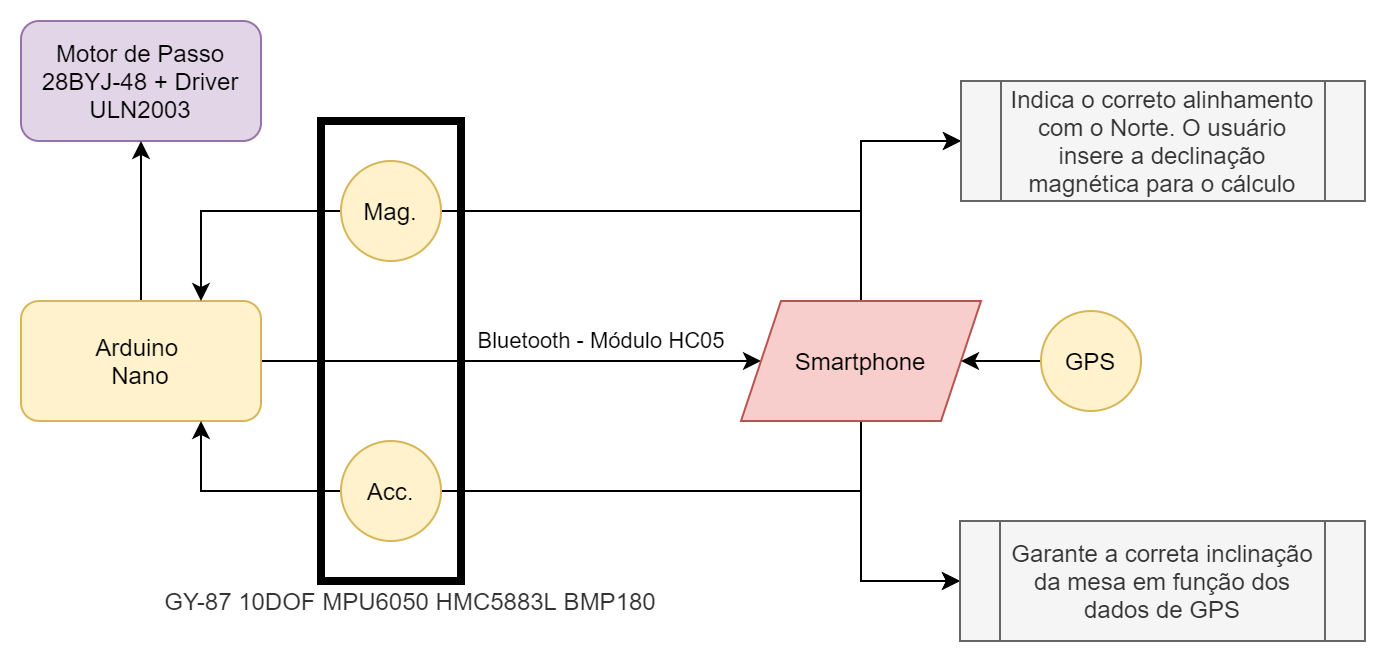
\includegraphics[width=0.8\linewidth]{imagens/PRJ_AFT_TCC-Page-2}
	\caption{Diagrama do sistema sem usar os sensores do \textit{smarptphone}}
	\label{fig:prjafttcc-page-1}
\end{figure}


A segunda é assumindo que o celular possua sensores.(Figura \ref{fig:prjafttcc-page-2}) Usando eles é possível minimizar o custo do produto em até 100 reais (GY87+HC05+Frete). Implementar isso, na verdade, não exige um trabalho enorme extra a princípio, pois independente de quem captar os dados, o importante é quem pode fazer todos os cálculos para colaborar com o usuário. No caso é o \textit{smartphone}. Saliento que ele deve ser facilmente fixável na mesa par que o alinhamento ocorra de forma correta.

\begin{figure}[!htb]
	\centering
	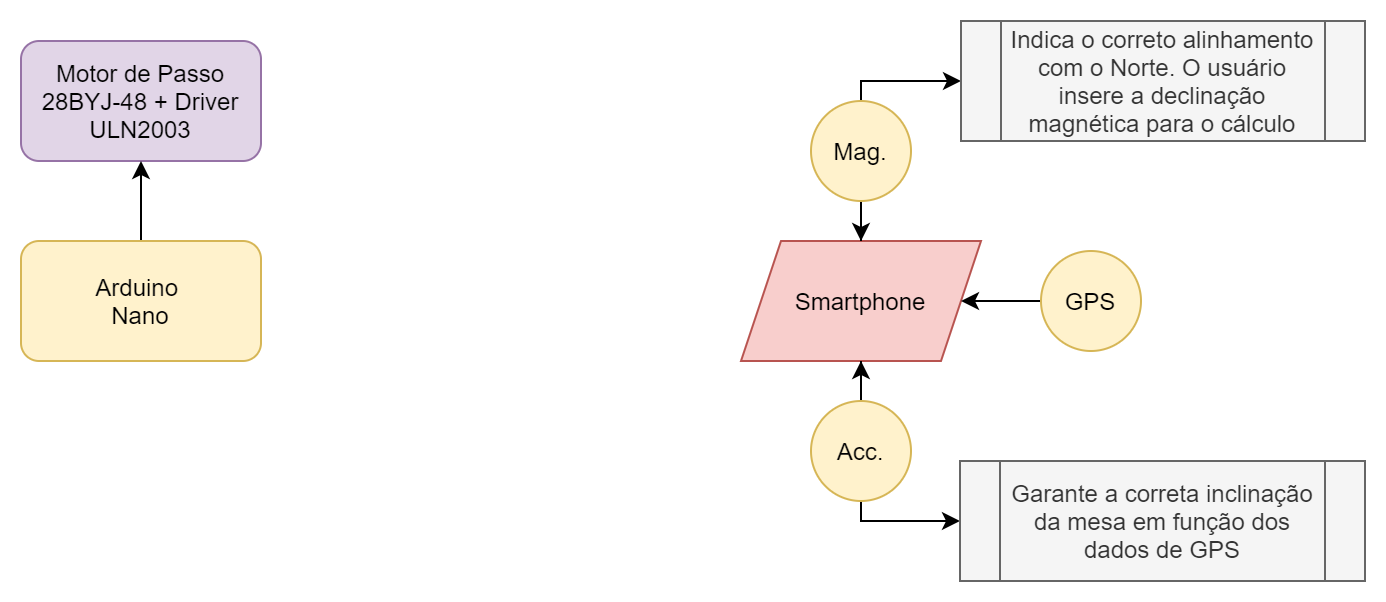
\includegraphics[width=0.8\linewidth]{imagens/PRJ_AFT_TCC-Page-1}
	\caption{Diagrama do sistema usando os sensores do \textit{smarptphone}}
	\label{fig:prjafttcc-page-2}
\end{figure}

Como os sensores do Arduino e os sensores do \textit{smartphone} possuam uma forma de funcionamento semelhante (em código), é possível fazer um código de aplicativo que funcione para ambos os cenários e a placa do sistema eletrônico também seja funcional em ambas as situações.

\section{Próximas Atividades}

Seguindo o Cronograma, a próxima atividade será a conclusão do CAD da mesa \textit{barn-door}. A \href{https://docs.google.com/spreadsheets/d/1AbPNhJbIAHxrgyp-HbyYSLwaWb71SL8_rIbzwGyOWhE/edit?usp=sharing}{tabela neste link}, que ainda estou completando e aprimorando,
ilustra a situação das peças em todas as fases de projeto e será o guia para a realização do CAD e posterior fabricação do sistema. 

O motor a ser utilizado e seu \textit{driver} já foram testados. Porém a eletrônica em si será inteiramente testada, definida e desenvolvida após a chegada dos demais componentes comprados. A tabela ora mencionada acima também indica a situação dos componentes. 

\end{document}